\documentclass{standalone}
\usepackage{tikz}

\begin{document}
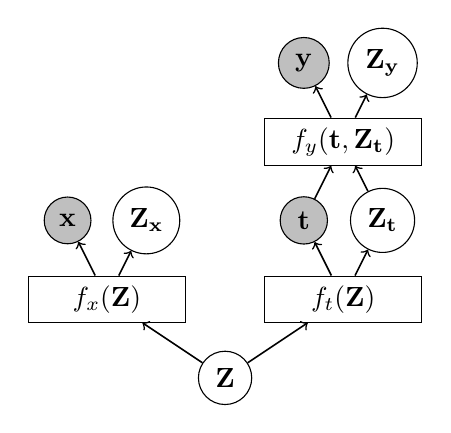
\begin{tikzpicture}
    \node[circle, draw=black, fill=lightgray] (x) at (-1, 0) {$\mathbf{x}$};
    \node[circle, draw=black, fill=white] (zx) at (0, 0) {$\mathbf{Z_x}$};
    \node[circle, draw=black, fill=white] (zt) at (3, 0) {$\mathbf{Z_t}$};
    \node[circle, draw=black, fill=lightgray] (t) at (2, 0) {$\mathbf{t}$};
    \node[circle, draw=black, fill=lightgray] (y) at (2, 2) {$\mathbf{y}$};
    \node[circle, draw=black, fill=white] (zy) at (3, 2) {$\mathbf{Z_y}$}; 
    \node[circle, draw=black, fill=white]  (z) at (1, -2) {$\mathbf{Z}$};
    
    \node[draw=black, minimum width=2cm] (fx) at (-0.5, -1) {$f_x(\mathbf{Z})$};
    \node[draw=black, minimum width=2cm] (ft) at (2.5, -1)  {$f_t(\mathbf{Z})$};
    \node[draw=black, minimum width=2cm] (fy) at (2.5, 1)  {$f_y(\mathbf{t}, \mathbf{Z_t})$};
    
    \draw[->, line width=0.2mm] (z) -- (fx);
    \draw[->, line width=0.2mm] (z) -- (ft);
    \draw[->, line width=0.2mm] (fx) -- (x);
    \draw[->, line width=0.2mm] (fx) -- (zx);
    \draw[->, line width=0.2mm] (ft) -- (t);
    \draw[->, line width=0.2mm] (ft) -- (zt);
    \draw[->, line width=0.2mm] (t) -- (fy);
    \draw[->, line width=0.2mm] (zt) -- (fy);
    \draw[->, line width=0.2mm] (fy) -- (y);
    \draw[->, line width=0.2mm] (fy) -- (zy);

\end{tikzpicture}
\end{document}